% ============================================================================================
% BAB III ANALISIS MASALAH
% Pembagian subbab tidak rigid dan dapat bervariasi. Bab ini minimal berisi analisis kebutuhan
% fungsional dan nonfungsional, analisis berbagai alternatif solusi yang dapat ditawarkan, dan
% metode pemilihan solusi yang diusulkan.
% ============================================================================================
\cleardoublepage
\chapter{ANALISIS MASALAH}
\label{chap:analisis-masalah}
\section{Analisis Kondisi Saat Ini}
\label{subsec:validasi-wawancara}
Bagian ini menganalisis permasalahan yang muncul dalam proses pengembangan sistem \textit{cloud-native} berbasis Kubernetes, ditinjau dari dua sudut utama, yaitu pemahaman masalah bisnis (\textit{Business Understanding}) dan kondisi data yang menjadi sumber permasalahan (\textit{Data Understanding}). Untuk memastikan permasalahan yang dirumuskan bersifat valid dan bukan sekadar asumsi teoritis, analisis ini dibangun atas triangulasi tiga jenis bukti, yaitu data sekunder berupa survei industri dan studi empiris terpublikasi, data primer berupa wawancara praktisi, serta analisis langsung terhadap spesifikasi OpenAPI Kubernetes.

\subsection{Pemahaman Masalah Bisnis (\textit{Business Understanding})}
Transformasi digital di berbagai industri mendorong adopsi arsitektur \textit{cloud-native} berbasis \textit{microservices} yang dikelola melalui Kubernetes. Dalam praktiknya, Kubernetes tidak hanya berfungsi sebagai alat operasional, tetapi juga sebagai aset strategis yang menentukan kecepatan dan stabilitas siklus pengembangan perangkat lunak (\textit{software development lifecycle}). Kompleksitas konfigurasi yang tinggi, kurva pembelajaran yang curam, serta kebutuhan untuk melakukan \textit{onboarding} bagi \textit{engineer} baru menjadikan Kubernetes sebuah titik krusial dalam kapasitas operasional.

Permasalahan terkait pengelolaan konfigurasi Kubernetes tidak hanya bersifat teknis, tetapi menimbulkan dampak bisnis berupa biaya operasional dan risiko produksi. Beberapa permasalahan utama yang diidentifikasi adalah sebagai berikut:

\begin{enumerate}
    \item \textbf{B01 - Inefisiensi Waktu (\textit{Operational Cost})} \\
    Dokumentasi Kubernetes bersifat luas dan terfragmentasi sehingga \textit{developer/DevOps} membutuhkan waktu yang cukup lama untuk menelusuri relasi antarobjek Kubernetes. Survei industri mencatat bahwa kerumitan konfigurasi YAML menjadi hambatan skalabilitas utama bagi mayoritas pengguna Kubernetes \parencite{cncf_2023_survey}. Beban ini bersifat struktural, sebagaimana ditunjukkan oleh analisis spesifikasi pada Subbab~\ref{subsec:eda} yang mengungkap bahwa hampir 60\% definisi skema saling bergantung melalui referensi silang. Temuan ini diperkuat wawancara praktisi yang melaporkan penggunaan asisten LLM secara intensif dalam pekerjaan harian, sebagian mencapai 15--20 kueri per hari, untuk menelusuri relasi dan mencari konteks konfigurasi. Waktu pencarian informasi yang berlebih menjadi pemborosan sumber daya, terutama pada posisi \textit{engineer} dengan biaya tenaga kerja tinggi.

    \item \textbf{B02 - Kesenjangan Pengetahuan (\textit{Knowledge Gap})} \\
    Dokumentasi statis tidak sepenuhnya mendukung cara berpikir asosiatif manusia ketika memahami struktur spesifikasi. Sistem generatif berbasis LLM pun masih sering menghasilkan \textit{hallucinated fields} karena tidak memiliki pemahaman skematik. Halusinasi merupakan fenomena yang terdokumentasi dan terukur pada model generatif \parencite{ji_hallucination_2023}, dan studi empiris terhadap pembuatan kode oleh LLM menunjukkan tingkat ketidaktepatan yang signifikan pada keluaran teknis \parencite{liu2024deepanalysis}. Wawancara praktisi mengonfirmasi pola ini secara konsisten, yaitu jawaban LLM yang gagal dijalankan, berbeda antarmodel, serta membuat asumsi yang tidak sesuai konteks pengguna. Hal ini dapat memperburuk risiko kesalahan konfigurasi.

    \item \textbf{B03 - Risiko Kesalahan Konfigurasi (\textit{Operational Risk})} \\
    Kesalahan sintaksis atau penempatan atribut berkas konfigurasi YAML yang tidak sesuai spesifikasi dapat menyebabkan \textit{deployment failure} hingga \textit{downtime}. Studi empiris terhadap manifes Kubernetes \textit{open-source} menemukan bahwa mayoritas miskonfigurasi bersifat struktural sehingga dapat dideteksi melalui analisis statis \parencite{rahman2023misconfigurations}. \textit{Downtime} produksi berimplikasi langsung pada kerugian finansial, reputasi layanan, dan penundaan proses bisnis. Praktisi mengonfirmasi risiko ini melalui pengalaman keluaran YAML yang tidak konsisten serta konfigurasi yang tidak memperbarui variabel terbaru.

\end{enumerate}

Ketiga butir \textit{business understanding} tersebut menjadi dasar dalam penyusunan rumusan masalah penelitian. Poin B01 mengenai inefisiensi waktu akibat dokumentasi yang terfragmentasi menunjukkan adanya kebutuhan terhadap representasi pengetahuan yang lebih terstruktur. Hal ini dirumuskan menjadi Rumusan Masalah 1, yaitu pembangunan \textit{knowledge graph} dari spesifikasi OpenAPI Kubernetes guna memetakan objek dan relasi hierarkis antarobjek konfigurasi secara komprehensif. Sementara itu, poin B02 yang menyoroti kesenjangan pemahaman skematik dan risiko \textit{hallucination} pada LLM, serta poin B03 mengenai risiko kesalahan konfigurasi akibat ketidaklengkapan atribut wajib YAML, secara bersama-sama mendasari Rumusan Masalah 2. Rumusan masalah ini difokuskan pada perancangan mekanisme GraphRAG yang memanfaatkan representasi struktural \textit{knowledge graph} melalui penelusuran jalur relasional (\textit{intent-adaptive depth traversal}) untuk meningkatkan kualitas \textit{retrieval}. Selanjutnya, penelitian ini akan mengidentifikasi keunggulan GraphRAG dibandingkan dengan Vector RAG dan Vanilla LLM dalam menyelesaikan berbagai persoalan yang telah diidentifikasi pada B01--B03.

\subsection{Pemahaman Data (\textit{Data Understanding})}
Bagian ini menjelaskan karakteristik data dokumentasi API Kubernetes yang menjadi sumber utama dalam proses konstruksi \textit{Graph-based Retrieval Augmentation}. Analisis mencakup identitas data, struktur, pola hubungan antarobjek Kubernetes, keterbatasan kualitas, serta seleksi data relevan yang digunakan dalam penelitian.

    \subsubsection{Sumber dan Spesifikasi Data (\textit{Data Source \& Specifications})}
    Data penelitian diperoleh dari repositori resmi Kubernetes pada GitHub \texttt{kubernetes/kubernetes}. Data diambil dalam bentuk berkas \texttt{swagger.json} yang mengikuti standar \textit{OpenAPI Specification} (OAS). Penelitian ini menggunakan versi Kubernetes \textbf{v1.30} sebagai acuan. Berkas \texttt{swagger.json} memiliki ukuran rata-rata 3,757 MB dan memuat 2.500--3.500 definisi API. Kompleksitas tersebut menjustifikasi penggunaan metode ekstraksi otomatis karena pendekatan manual berpotensi menghasilkan kesalahan interpretasi struktur dan kehilangan relasi semantik antarobjek Kubernetes.

    \subsubsection{Analisis Struktur Dokumen}
    Berdasarkan analisis terhadap struktur \texttt{swagger.json}, terdapat dua komponen utama beserta karakteristik hierarkisnya:
    \begin{enumerate}
        \item \textbf{\textit{Definitions} (atau \textit{Schema Resources}):} Mendeskripsikan spesifikasi objek Kubernetes seperti \textit{Pod}, \textit{Service}, dan \textit{Deployment}. Hampir seluruh objek Kubernetes mematuhi pola struktural wajib yang terdiri atas \texttt{apiVersion}, \texttt{kind}, \texttt{metadata}, \texttt{spec}, dan \texttt{status}. Namun, isi dari atribut \texttt{spec} sangat bervariasi antarkomponen di dalam teks YAML. Akibatnya, waktu pembuatan konfigurasi meningkat dan pengembang sangat bergantung pada panduan eksternal. Secara spesifik, setiap definisi skema di bagian ini memuat:
        \begin{enumerate}[a.]
            \item \texttt{properties}: Merepresentasikan \textit{field} aktual pada berkas konfigurasi YAML.
            \item \texttt{type}: Menentukan format tipe data (seperti \textit{object, array, string, integer, boolean}).
            \item \texttt{required}: Mendefinisikan daftar \textit{field} konfigurasi yang wajib diisi.
            \item \texttt{description}: Menyediakan dokumentasi tekstual mengenai fungsionalitas \textit{field}.
            \item \texttt{\$ref}: Bertindak sebagai referensi silang ke definisi skema bersarang (\textit{nested schema}). Ciri utama struktur dokumen ini adalah ketergantungan referensial bersarang antardefinisi skema sehingga satu \textit{field} YAML dapat mengarah ke objek skema lain, struktur daftar (\textit{array}), maupun struktur pemetaan (\textit{map}). Ketiga bentuk referensi ini dianalisis lebih lanjut pada Subbab~\ref{subsec:keterhubungan-data}.
        \end{enumerate}

        \item \textbf{\textit{Paths}:} Mendeskripsikan \textit{endpoint} API, misalnya \texttt{GET /api/v1/pods}, sebagai antarmuka interaksi objek Kubernetes dalam ekosistem klaster. Setiap \textit{endpoint} memiliki atribut penentu interaksi komunikasi yang memuat:
        \begin{enumerate}[a.]
            \item Metode HTTP fungsional (\textit{GET, POST, PUT, PATCH, DELETE}).
            \item Parameter injeksi pada jalur (\textit{path}) dan kueri (\textit{query}).
            \item Skema respons (\textit{response schema}) dari \textit{server}.
            \item Relasi struktural pembentuk fungsionalitas yang mengarah kembali ke blok \texttt{definitions}.
        \end{enumerate}
    \end{enumerate}

    \subsubsection{Analisis Data Eksploratif Spesifikasi OpenAPI}
    \label{subsec:eda}

        Sebelum merancang skema \textit{knowledge graph}, analisis data eksploratif (\textit{Exploratory Data Analysis} / EDA) dilakukan terhadap berkas \texttt{kubernetes\_swagger.json} berukuran 3,757 MB guna memetakan skala, kompleksitas struktural, dan sebaran definisi skema. Proses ekstraksi awal berhasil mengidentifikasi 735 definisi skema. Sebanyak 5 entri diabaikan karena teridentifikasi sebagai \textit{noise}, menyisakan 730 definisi skema valid untuk dievaluasi lebih lanjut.

        Temuan utama dari proses EDA ini dikelompokkan ke dalam dua metrik utama:

        \begin{enumerate}
            \item \textbf{Distribusi objek Kubernetes \textit{root} vs komponen pendukung}\\
            Klasifikasi definisi skema menunjukkan ketimpangan proporsi yang sangat signifikan antara objek utama dan objek pendukung. Dari total 730 definisi, hanya 183 (24,9\%) terklasifikasi sebagai objek Kubernetes \textit{root} (\textit{root resources}). Objek \textit{root} ini merupakan objek yang memiliki atribut \textit{GroupVersionKind} (GVK) sehingga dapat diterapkan secara langsung ke dalam klaster. Sementara itu, sebagian besar definisi (547 definisi atau 75,1\%) merupakan skema pendukung (\textit{sub-resources}) yang menyusun komponen \textit{root} tersebut. Ketimpangan ini menunjukkan besarnya dependensi struktural di dalam Kubernetes.
                \begin{figure}[H]
                    \centering
                    \captionsetup{justification=centering}
                    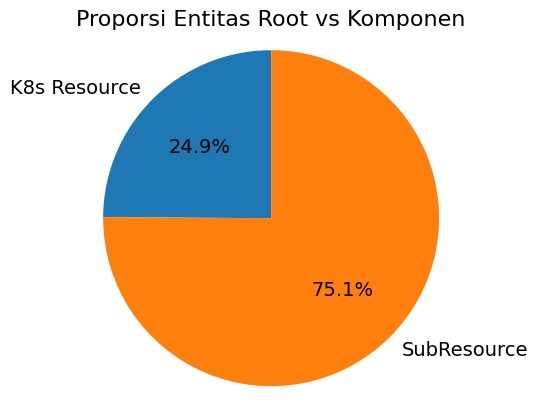
\includegraphics[width=1.00\textwidth]{images/Proporsi-root-komponen.jpeg}
                    \caption{Proporsi objek Kubernetes \textit{root} vs komponen pendukung dalam spesifikasi OpenAPI Kubernetes}
                    \label{fig:kubernetes-root-proportion}
                \end{figure}

            \item \textbf{Kepadatan Properti dan Intensitas Referensi Silang}\\
            Inspeksi terhadap struktur properti mengungkap bahwa setiap definisi skema rata-rata memuat 4,1 atribut konfigurasi (\textit{field}) dengan objek Kubernetes paling kompleks menampung hingga 44 atribut. Selain itu, ditemukan bahwa 437 dari 730 definisi (59,9\%) tercatat memuat setidaknya satu referensi ke skema lain melalui mekanisme \texttt{\$ref}. Temuan ini mengindikasikan bahwa pemahaman terhadap satu objek Kubernetes menuntut penelusuran ke definisi skema lain sehingga penulisan konfigurasi secara manual menjadi semakin kompleks.
        \end{enumerate}

    \subsubsection{Analisis Keterhubungan Data}
    \label{subsec:keterhubungan-data}
        Secara struktural, keterhubungan antardefinisi pada \texttt{swagger.json} dinyatakan melalui mekanisme referensi silang (\texttt{\$ref}). Sebuah properti pada satu definisi skema dapat merujuk definisi lain dalam tiga bentuk, yaitu referensi langsung ke objek skema lain, referensi di dalam struktur daftar (\textit{array}), serta referensi di dalam struktur pemetaan (\textit{map}). Ketiga bentuk inilah yang menjadi sumber deterministik bagi pembentukan \textit{edge} struktural pada graf.

        \begin{enumerate}[a.]
            \item \textbf{Referensi ke objek skema lain}\\
            Properti merujuk satu objek skema lain secara langsung. Sebagai contoh, properti \texttt{selector} pada \textit{DaemonSetSpec} merujuk definisi \textit{LabelSelector} sehingga isi di bawah \texttt{selector} mengikuti struktur \textit{LabelSelector}, sebagaimana Kode~\ref{lst:ref-object} dan \ref{lst:ref-object-yaml}.
\begin{lstlisting}[language=bash, frame=single, caption={Skema referensi objek pada \texttt{swagger.json}}, captionpos=t, label={lst:ref-object}]
"selector": {
  "$ref": "#/definitions/io.k8s.apimachinery.pkg.apis.meta.v1.LabelSelector"
}
\end{lstlisting}
\begin{lstlisting}[language=bash, frame=single, caption={Wujud YAML objek \textit{LabelSelector}}, captionpos=t, label={lst:ref-object-yaml}]
selector:              # nilai berbentuk objek LabelSelector
  matchLabels:         # field milik LabelSelector
    app: nginx
\end{lstlisting}

            \item \textbf{Referensi di dalam struktur daftar (\textit{array})}\\
            Properti bertipe \texttt{array} merujuk definisi skema melalui atribut \texttt{items}. Sebagai contoh, properti \texttt{containers} pada \textit{PodSpec} memuat daftar objek \textit{Container} dengan tiap elemen bertipe \textit{Container} dan dibedakan oleh urutannya, sebagaimana Kode~\ref{lst:ref-array} dan \ref{lst:ref-array-yaml}.
\begin{lstlisting}[language=bash, frame=single, caption={Skema referensi daftar pada \texttt{swagger.json}}, captionpos=t, label={lst:ref-array}]
"containers": {
  "type": "array",
  "items": {
    "$ref": "#/definitions/io.k8s.api.core.v1.Container"
  }
}
\end{lstlisting}
\begin{lstlisting}[language=bash, frame=single, caption={Wujud YAML daftar objek \textit{Container}}, captionpos=t, label={lst:ref-array-yaml}]
containers:            # array; tiap elemen objek Container
  - name: app          # Container ke-1 (name = field Container)
    image: nginx:1.25
  - name: sidecar      # Container ke-2, dibedakan oleh urutan
    image: envoy:v1.31
\end{lstlisting}

            \item \textbf{Referensi di dalam struktur pemetaan (\textit{map})}\\
            Properti bertipe \texttt{object} merujuk definisi skema melalui atribut \texttt{additional Properties}. Sebagai contoh, properti \texttt{limits} pada \textit{ResourceRequirements} memetakan setiap kunci ke objek \textit{Quantity} dengan nama kunci dipilih bebas oleh pengguna, sebagaimana Kode~\ref{lst:ref-map} dan \ref{lst:ref-map-yaml}.
\begin{lstlisting}[language=bash, frame=single, caption={Skema referensi pemetaan pada \texttt{swagger.json}}, captionpos=t, label={lst:ref-map}]
"limits": {
  "type": "object",
  "additionalProperties": {
    "$ref": "#/definitions/io.k8s.apimachinery.pkg.api.resource.Quantity"
  }
}
\end{lstlisting}
\begin{lstlisting}[language=bash, frame=single, caption={Wujud YAML pemetaan objek \textit{Quantity}}, captionpos=t, label={lst:ref-map-yaml}]
limits:                # map; tiap nilai objek Quantity
  cpu: "500m"          # kunci 'cpu' (bebas), nilai Quantity
  memory: "1Gi"        # kunci 'memory' (bebas), nilai Quantity
\end{lstlisting}
        \end{enumerate}

\section{Analisis Kebutuhan}
Tahap analisis kebutuhan berfokus pada identifikasi kapabilitas yang harus
dimiliki sistem guna menjawab tujuan penelitian dan kebutuhan bisnis. Untuk memastikan kebutuhan yang dirumuskan relevan dengan masalah yang dihadapi, penelitian ini menganalisis kesenjangan teknis (\textit{technical gap}) pendekatan \textit{Retrieval-Augmented Generation} yang ada, termasuk pendekatan GraphRAG pada domain teknis serupa \parencite{civiot2025graphrag, hsgrag2025acm}. Hasil analisis disajikan pada Tabel~\ref{tbl:comparison_existing_graphRAG}.
\renewcommand{\arraystretch}{1.25}
\captionsetup[longtable]{justification=raggedright,singlelinecheck=false}

\begin{longtable}{|p{3cm}|p{5cm}|p{5cm}|}
\caption{\textit{Technical Gap Analysis} pada Domain Kubernetes}
\label{tbl:comparison_existing_graphRAG} \\ \hline
\multicolumn{1}{|p{3cm}|}{\centering\textbf{Aspek Kesenjangan Teknis}} &
\multicolumn{1}{p{5cm}|}{\centering\textbf{Kondisi Saat Ini (\textit{Existing Approaches})}} &
\multicolumn{1}{p{5cm}|}{\centering\textbf{Kesenjangan di Domain Kubernetes}} \\ \hline
\endfirsthead

\multicolumn{3}{l}{Tabel \ref{tbl:comparison_existing_graphRAG} \textit{Technical Gap Analysis} pada Domain Kubernetes (lanjutan)} \\ \hline
\multicolumn{1}{|p{3cm}|}{\centering\textbf{Aspek Kesenjangan Teknis}} &
\multicolumn{1}{p{5cm}|}{\centering\textbf{Kondisi Saat Ini (\textit{Existing Approaches})}} &
\multicolumn{1}{p{5cm}|}{\centering\textbf{Kesenjangan di Domain Kubernetes}} \\ \hline
\endhead

\hline
\multicolumn{3}{r}{\textit{bersambung ke halaman berikutnya}} \\
\endfoot

\hline
\endlastfoot

T01 - Representasi Struktur Data &
Menggunakan pemecahan teks secara \textit{linear chunking} ataupun konstruksi \textit{knowledge graph} berbasis ekstraksi entitas generik dari teks, tanpa mendefinisikan taksonomi jenis relasi yang spesifik terhadap semantik domain target \parencite{cao2025neusymrag, civiot2025graphrag, hsgrag2025acm}. &
Terjadi kehilangan konteks mendalam (\textit{loss of deep context}) dan ambiguitas semantik relasi. Sistem gagal memahami kedalaman hierarki bersarang (misalnya properti \texttt{limits} sebagai turunan dari \textit{Deployment}) sekaligus tidak dapat membedakan jenis relasi antar-objek Kubernetes. \\ \hline

T02 - Mekanisme Validasi &
Validasi bergantung pada model LLM atau aturan manual berbasis \textit{hard constraints} yang harus ditulis satu per satu \parencite{wan2025empowering}. &
Risiko terjadinya \textit{syntactic hallucination} tinggi (LLM mengarang \textit{field}), atau beban pemeliharaan menjadi besar saat aturan manual harus diperbarui \parencite{rag_survey}. \\ \hline

T03 - Ambiguitas Entitas &
Mengandalkan frekuensi kemunculan kata kunci (\textit{keyword frequency}) atau kedekatan vektor semata \parencite{rag_survey}. &
Terdapat ambiguitas pada pola \textit{loose coupling} karena \textit{keywords} (misal: \textit{labels}, \textit{ports}) muncul berulang di banyak objek berbeda. Hal ini menyebabkan tercampurnya konteks antar-objek (\textit{contextual mixing}) \parencite{kotstein_restberta_2024}. \\ \hline

T04 - Pemeliharaan Pengetahuan &
Membutuhkan \textit{fine-tuning} ulang model atau pembaruan aturan manual ketika terjadi perubahan versi API \parencite{rag_survey}. Penelitian GraphRAG terkini pada domain teknis serupa pun masih menghadapi keterbatasan yang sama berupa \textit{knowledge graph} yang bersifat statis tanpa mekanisme pembaruan dinamis \parencite{civiot2025graphrag, hsgrag2025acm}. &
Tidak efisien, mudah menjadi \textit{obsolete}, dan sensitif terhadap perubahan versi Kubernetes yang dirilis secara berkala. \\ \hline

T05 - Akurasi Jawaban &
Sistem cenderung menghasilkan jawaban naratif dan tidak memberikan jaminan presisi sintaksis konfigurasi YAML \parencite{liu2024deepanalysis}. &
Tidak mampu menghasilkan artefak konfigurasi yang sesuai karena sering ditemukan kesalahan format atau struktur \parencite{rahman2023misconfigurations}. \\ \hline

\end{longtable}

\subsection{Kebutuhan Fungsional}
Berdasarkan \textit{Business Understanding} (B01--B03), diidentifikasi sejumlah
urgensi bisnis yang dianalisis lebih lanjut hingga menghasilkan beberapa
kesenjangan teknis (T01--T05) yang menjadi dasar perumusan kebutuhan sistem.
Setiap kesenjangan teknis kemudian dijawab melalui
perancangan kebutuhan fungsional yang akan
diimplementasikan untuk menyelesaikan permasalahan bisnis yang ada.
Tabel \ref{tbl:mapping_business_gap_functional} berikut memetakan hubungan antara kebutuhan bisnis, kesenjangan teknis, serta kebutuhan fungsional yang dirumuskan untuk mengatasinya.

\captionsetup[table]{justification=raggedright,singlelinecheck=false}
\begin{table}[H]
\centering
\renewcommand{\arraystretch}{1.25}
\begin{tabular}{|
    >{\raggedright\arraybackslash}p{4cm}|
    >{\raggedright\arraybackslash}p{3.5cm}|
    >{\raggedright\arraybackslash}p{5cm}|
}
\hline
\multicolumn{1}{|p{4cm}|}{\textbf{Business Requirement (B)}} &
\multicolumn{1}{p{3.5cm}|}{\textbf{Technical GAP (T)}} &
\multicolumn{1}{p{5cm}|}{\textbf{Functional Requirement (F)}} \\ \hline

% ===== B01 =====
\multirow{5}{4cm}{\textbf{B01} -- Inefisiensi waktu}
  & \multirow{2}{3.5cm}{\textbf{T01} -- Representasi struktur data}
    & \textbf{F-01} \textit{Structured Object Representation} \\ \cline{3-3}
  &  & \textbf{F-02} \textit{Structured Relation Retrieval} \\ \cline{2-3}

  & \multirow{3}{3.5cm}{\textbf{T03} -- Ambiguitas entitas}
    & \textbf{F-03} \textit{Intent Classification} \\ \cline{3-3}
  &  & \textbf{F-04} \textit{Context Construction \& Injection} \\ \cline{3-3}
  &  & \textbf{F-05} \textit{Semantic Embedding} \\ \hline

% ===== B02 =====
\multirow{2}{4cm}{\textbf{B02} -- Kesenjangan pengetahuan}
  & \textbf{T02} -- Mekanisme validasi
    & \textbf{F-07} \textit{Conditional YAML Generation Constraint} \\ \cline{2-3}
  & \textbf{T04} -- Pemeliharaan pengetahuan
    & \textbf{F-01} \textit{Structured Object Representation} \\ \hline

% ===== B03 =====
\multirow{2}{4cm}{\textbf{B03} -- Risiko kesalahan konfigurasi}
  & \multirow{2}{3.5cm}{\textbf{T05} -- Akurasi jawaban}
    & \textbf{F-06} \textit{Web Interaction Interface} \\ \cline{3-3}
  &  & \textbf{F-07} \textit{Conditional YAML Generation Constraint} \\ \hline

\end{tabular}
\caption{Pemetaan Kebutuhan Bisnis terhadap \textit{Technical Gap} dan Kebutuhan Fungsional}
\label{tbl:mapping_business_gap_functional}
\end{table}

Berdasarkan hasil pemetaan pada Tabel \ref{tbl:mapping_business_gap_functional}, berikut adalah kebutuhan fungsional yang harus dipenuhi sistem,
\captionsetup[longtable]{justification=raggedright,singlelinecheck=false}

\begin{longtable}{ | p{0.1\textwidth} | p{0.30\textwidth} | p{0.50\textwidth} |}
\caption{Kebutuhan Fungsional Sistem}
\label{tbl:fungsional} \\
\hline
\multicolumn{1}{|p{0.1\textwidth}|}{\centering\textbf{Kode}} & \multicolumn{1}{p{0.30\textwidth}|}{\centering\textbf{Parameter}} & \multicolumn{1}{p{0.50\textwidth}|}{\centering\textbf{Deskripsi Spesifikasi}} \\
\hline
\endfirsthead

\multicolumn{3}{l}{Tabel \ref{tbl:fungsional} Kebutuhan Fungsional Sistem (lanjutan)} \\
\hline
\multicolumn{1}{|p{0.1\textwidth}|}{\centering\textbf{Kode}} & \multicolumn{1}{p{0.30\textwidth}|}{\centering\textbf{Parameter}} & \multicolumn{1}{p{0.50\textwidth}|}{\centering\textbf{Deskripsi Spesifikasi}} \\
\hline
\endhead


\hline
\multicolumn{3}{r}{\textit{bersambung ke halaman berikutnya}} \\
\endfoot

\hline
\endlastfoot

F-01 & \textit{Structured Object Representation} & Sistem harus mengubah skema objek ke dalam suatu representasi terstruktur yang membedakan setiap komponen, \textit{field}, dan relasi antar-objek sehingga dapat diakses kembali secara terprogram pada tahap \textit{retrieval}. \\
\hline

F-02 & \textit{Structured Relation Retrieval} & Sistem harus menyediakan mekanisme \textit{retrieval} yang mampu mengambil himpunan objek dan \textit{field} yang saling berkaitan (misalnya hubungan antara \textit{Deployment}, \textit{Pod}, dan \textit{Service}) berdasarkan entitas awal dan \textit{intent} pengguna sebagaimana didefinisikan pada F-03. \\
\hline

F-03 & \textit{Intent Classification} & Sistem harus mampu (1) mendeteksi entitas Kubernetes yang dirujuk pengguna (misalnya \textit{Service}, \textit{Pod}), dan (2) mengklasifikasikan maksud pengguna ke dalam beberapa kategori kueri yang berbeda sehingga strategi \textit{retrieval} dan format keluaran dapat disesuaikan dengan karakteristik tiap jenis kueri. \\
\hline

F-04 & \textit{Context Construction \& Injection} & Sistem harus mengubah hasil F-02 menjadi konteks terstruktur yang dapat digunakan sebagai basis generasi jawaban. \\
\hline

F-05 & \textit{Semantic Embedding} & Sistem harus menghasilkan representasi vektor (\textit{embedding}) untuk setiap node dalam representasi terstruktur dan menyimpannya ke dalam indeks vektor, sehingga pencarian berbasis kemiripan semantik dapat digunakan sebagai mekanisme \textit{fallback} pada tahap \textit{retrieval}. \\
\hline

F-06 & \textit{Web Interaction Interface} &
Sistem harus menyediakan antarmuka web interaktif yang memungkinkan pengguna memasukkan pertanyaan dalam bahasa alami, menampilkan jawaban beserta konfigurasi YAML (jika relevan), serta menyajikan jejak penalaran (\textit{reasoning path}) secara visual disertai pesan kesalahan yang informatif. \\
\hline

F-07 & \textit{Conditional YAML Generation Constraint} & Sistem harus secara kondisional menghasilkan keluaran berupa blok kode YAML yang valid secara sintaksis apabila pengguna meminta pembuatan konfigurasi, dan menghasilkan jawaban naratif untuk jenis kueri lainnya yang tidak bersifat generatif. \\
\hline


\end{longtable}


\subsection{Kebutuhan Non Fungsional}
Kebutuhan non-fungsional mendefinisikan karakteristik kualitas yang harus dimiliki oleh sistem untuk memastikan kinerja, keandalan, dan keamanan operasional. Kebutuhan ini penting untuk menjamin bahwa sistem tidak hanya berfungsi dengan benar, tetapi juga memenuhi standar kualitas yang diharapkan oleh pengguna. Berikut adalah kebutuhan non-fungsional utama yang diidentifikasi:
\captionsetup[longtable]{justification=raggedright,singlelinecheck=false}

\begin{longtable}{ | p{0.1\textwidth} | p{0.30\textwidth} | p{0.50\textwidth} |}
\caption{Kebutuhan Non-Fungsional Sistem}
\label{tbl:nonfungsional} \\
\hline
\multicolumn{1}{|p{0.1\textwidth}|}{\centering\textbf{Kode}} & \multicolumn{1}{p{0.30\textwidth}|}{\centering\textbf{Parameter}} & \multicolumn{1}{p{0.50\textwidth}|}{\centering\textbf{Deskripsi Spesifikasi}} \\
\hline
\endfirsthead

\multicolumn{3}{l}{Tabel \ref{tbl:nonfungsional} Kebutuhan Non-Fungsional Sistem (lanjutan)} \\
\hline
\multicolumn{1}{|p{0.1\textwidth}|}{\centering\textbf{Kode}} & \multicolumn{1}{p{0.30\textwidth}|}{\centering\textbf{Parameter}} & \multicolumn{1}{p{0.50\textwidth}|}{\centering\textbf{Deskripsi Spesifikasi}} \\
\hline
\endhead

\hline
\multicolumn{3}{r}{\textit{bersambung ke halaman berikutnya}} \\
\endfoot

\hline
\endlastfoot

NF-01 (\textit{Reliability}) & \textit{Fail-Safe Mechanism} &
Sistem harus mencegah keluaran halusinasi melalui mekanisme \textit{error handling}, yaitu (1) Jika entitas tidak ditemukan, sistem harus memberi respons ``Entity not found''. (2) Jika YAML terdeteksi tidak valid oleh validator internal, sistem harus menampilkan peringatan ``Warning: Potential Syntax Error'' pada antarmuka pengguna. \\
\hline
 
NF-02 (\textit{Performance}) & \textit{Retrieval--Generation Latency} & Waktu total yang dibutuhkan untuk memproses satu permintaan pengguna (\textit{end-to-end latency}) tidak boleh melebihi \textbf{60 detik} pada lingkungan pengujian standar. \\
\hline

NF-03 (\textit{Usability}) & \textit{Web UI Usability Standard} & Antarmuka web interaktif sistem harus menyediakan pengalaman penggunaan yang konsisten, mudah dipahami, dan informatif, mencakup mekanisme input pertanyaan, panel tampilan jawaban, serta visualisasi jejak penalaran. \\
\hline

NF-04 (\textit{Accessibility}) & \textit{Public Accessibility} &
Sistem harus dapat diakses oleh pengguna umum melalui antarmuka web yang tersedia secara daring, tanpa memerlukan instalasi perangkat lunak tambahan di sisi pengguna. \\ \hline

\end{longtable}

\subsection{Pemetaan Kebutuhan Bisnis terhadap Kerangka Evaluasi}

Untuk memastikan bahwa setiap dimensi evaluasi sistem memiliki dasar bisnis yang jelas, Tabel~\ref{tbl:mapping_bisnis_evaluasi} memetakan hubungan antara kebutuhan bisnis (B01--B03), dimensi evaluasi, dan metrik yang digunakan.

\renewcommand{\arraystretch}{1.1}
\captionsetup[table]{justification=raggedright,singlelinecheck=false}
\begin{table}[htbp]
\caption{Pemetaan kebutuhan bisnis terhadap dimensi dan metrik evaluasi}
\label{tbl:mapping_bisnis_evaluasi}
\centering
\begin{tabular}{| p{0.18\textwidth} | p{0.32\textwidth} | p{0.10\textwidth} | p{0.25\textwidth} |}
\hline
\textbf{Kebutuhan Bisnis} & \textbf{Pertanyaan Evaluasi} & \textbf{Dimensi} & \textbf{Metrik Utama} \\
\hline
B01 -- Inefisiensi Waktu & Apakah hasil \textit{retrieval} memiliki presisi tinggi dan mencakup relasi yang dibutuhkan sehingga meminimalisir penelusuran manual? & RetQ & Precision, Recall, F1 (\textit{set-based}, Manning 2008) \\
\hline
B02 -- Kesenjangan Pengetahuan & Apakah jawaban dapat ditelusuri ke konteks graf yang relevan, bukan dari pengetahuan parametrik model? & ReaQ & \textit{Hop Accuracy}, \textit{Faithfulness} \\
\hline
B03 -- Risiko Konfigurasi & Apakah keluaran YAML valid dan relevan terhadap kueri? & AnsQ & \textit{Syntactic Validity}, \textit{Schema Compliance}, \textit{Answer Semantic Similarity} \\
\hline
\end{tabular}
\end{table}


Pemetaan ini mempertegas bahwa dimensi evaluasi bukan sekadar metrik teknis, melainkan representasi langsung dari dampak bisnis yang ingin dimitigasi oleh sistem GraphRAG.

\section{Alternatif Solusi}
Bagian ini membahas berbagai alternatif solusi yang dapat diimplementasikan untuk memenuhi kebutuhan sistem yang telah diidentifikasi sebelumnya.

\subsection{Hybrid KG--Vector RAG}
Pendekatan \textit{hybrid KG--Vector RAG} menggabungkan dua jalur pencarian, yakni \textit{vector-based RAG} untuk pencarian semantik dan \textit{knowledge graph} (KG) berbasis metadata untuk penalaran relasional \parencite{wan2025empowering}. Kueri pengguna diproses melalui ekstraksi entitas untuk menarik subgraf relevan dari KG sekaligus mengambil potongan teks melalui pencarian kemiripan vektor; kedua konteks terstruktur dan semantik ini kemudian digabungkan sebagai basis generasi bagi LLM.

Hasil evaluasi oleh \textcite{wan2025empowering} pada dataset benchmark menunjukkan peningkatan yang signifikan dibanding \textit{vector-only RAG}: \textit{Exact Match} meningkat dari 63,4\% menjadi 77,8\% (+14,4 poin persentase) dan \textit{Context Precision} dari 69,8\% menjadi 76,5\% (+6,7 poin persentase). Konsekuensi dari penggabungan dua jalur ini adalah lonjakan latensi akibat \textit{traversal overhead} graf dan kompleksitas \textit{prompt engineering}.

\subsection{\textit{GNN-augmented GraphRAG} (G-Retriever)}
Arsitektur G-Retriever dirancang untuk menangani pemahaman graf tekstual berskala besar dengan memadukan \textit{Graph Neural Networks} (GNN) dan LLM \parencite{he2024gretriever}. Sistem ini mereduksi ukuran konteks kueri melalui algoritma \textit{Prize-Collecting Steiner Tree} (PCST) guna membangun subgraf koheren berisi \textit{node} dan \textit{edge} paling informatif sebelum disuntikkan ke dalam LLM.

Secara kuantitatif, pendekatan ini mampu memangkas penggunaan token hingga 99\% dibanding RAG konvensional, sekaligus menaikkan validitas \textit{node} dari 31\% menjadi \textbf{77\%} (+46 poin persentase) dan validitas \textit{edge} dari 12\% menjadi 76\% tanpa memerlukan proses \textit{fine-tuning} pada LLM \parencite{he2024gretriever}. Namun, metode PCST memiliki kompleksitas komputasi $O(|V| + |E|)$ yang semakin meningkat seiring ukuran graf, dan ketergantungan terhadap GNN menyebabkan \textit{indexing} harus diulang setiap versi Kubernetes berubah.

\subsection{\textit{Hybrid Neural-Symbolic} dengan \textit{Relational DB} (NeuSym-RAG)}
Metode NeuSym-RAG memadukan model neural dengan basis pengetahuan simbolik berbasis aturan di dalam basis data relasional \parencite{cao2025neusymrag}. Pendekatan ini menyimpan entitas dalam tabel terstruktur dan mengeksekusi aturan simbolik untuk memvalidasi hasil inferensi LLM secara deterministik dengan akurasi validasi mencapai lebih dari 90\% pada dataset \textit{question answering} terstruktur \parencite{cao2025neusymrag}.

Namun, skema penyimpanan relasional memiliki kelemahan struktural jika diaplikasikan pada domain Kubernetes. Dengan 730 definisi skema dan rata-rata 4,1 \textit{field} per definisi, menelusuri relasi hierarkis bersarang (\textit{multi-hop}) membutuhkan operasi \textit{join} SQL yang kompleks. Selain itu, aturan simbolik harus didefinisikan secara manual untuk setiap relasi dan diperbarui setiap siklus rilis Kubernetes (rata-rata setiap 4 bulan), menjadikan pemeliharaan tidak praktis dalam skala produksi.

\section{Analisis Pemilihan Solusi}
Bagian ini bertujuan menentukan pendekatan pemecahan masalah yang paling sesuai untuk membangun sistem \textit{Graph-based Retrieval} pada dokumentasi API Kubernetes. Evaluasi dilakukan dengan membandingkan beberapa alternatif solusi berdasarkan kriteria yang disesuaikan dengan karakteristik konfigurasi \textit{cloud-native} yang bersifat deklaratif, terstruktur, dan saling bergantung secara hierarkis.

\subsection{Rubrik Evaluasi Solusi}
Evaluasi dilakukan menggunakan skala 1 (Kurang Baik) hingga 5 (Sangat Baik), berdasarkan empat kriteria utama sebagai berikut:

\begin{enumerate}[label=\textbf{K\arabic*.}]
    \item \textbf{Kesesuaian Representasi Data} \\
    Mengukur kemampuan metode dalam menangani data konfigurasi yang bersifat hierarkis dan memiliki \textit{cross-reference} antarobjek Kubernetes (misalnya \textit{Service} $\rightarrow$ \textit{Pod} melalui \textit{selector}).

    \item \textbf{Kemampuan Generatif} \\
    Menilai kemampuan sistem menghasilkan berkas konfigurasi YAML yang baru dan valid, bukan sekadar menemukan lokasi informasi pada dokumentasi.

    \item \textbf{Fleksibilitas Pemeliharaan} \\
    Mengukur kemudahan sistem dalam melakukan pembaruan pengetahuan ketika spesifikasi API Kubernetes berubah versi tanpa memerlukan \textit{fine-tuning} ulang.

    \item \textbf{Presisi Konteks} \\
    Menilai kemampuan sistem menekan halusinasi melalui pembatasan struktural yang tegas, terutama pada relasi antarobjek Kubernetes.
\end{enumerate}

Tabel~\ref{tbl:rubrik_eval} menunjukkan kategori penilaian untuk setiap skor pada rubrik evaluasi tersebut.
\captionsetup[table]{justification=raggedright,singlelinecheck=false}

\begin{table}[htbp]
\centering
\caption{Rubrik Penilaian Kriteria Evaluasi Solusi}
\label{tbl:rubrik_eval}
\begin{tabular}{ p{0.1\textwidth} p{0.15\textwidth} p{0.65\textwidth} }
\hline
\textbf{Skor} & \textbf{Kategori} & \textbf{Deskripsi} \\
\hline
1 & Kurang Baik & Tidak memenuhi kebutuhan domain Kubernetes secara fungsional maupun struktural. \\ \hline
2 & Cukup Buruk & Hanya relevan sebagian dan berisiko tinggi menghasilkan kesalahan konfigurasi. \\ \hline
3 & Cukup Baik & Dapat digunakan, tetapi memerlukan banyak penyesuaian untuk konteks Kubernetes. \\ \hline
4 & Baik & Umumnya sesuai dan dapat diterapkan dengan penyesuaian minor. \\ \hline
5 & Sangat Baik & Sangat sesuai dengan karakteristik masalah dan hampir tidak memerlukan modifikasi. \\ \hline
\end{tabular}
\end{table}


\subsection{Matriks Keputusan \& Justifikasi Penilaian}
Penilaian dilakukan terhadap tiga pendekatan alternatif sebagai kandidat solusi menggunakan metode \textit{Weighted Sum Model} (WSM) dengan bobot setara ($w = 0{,}25$ per kriteria, $\Sigma w = 1{,}0$). Alternatif~1 (Hybrid KG--Vector RAG) merupakan pendekatan yang diusulkan dalam penelitian ini. Hasil evaluasi ditampilkan pada Tabel~\ref{tbl:matriks_solutions}.

\begin{longtable}{|
>{\raggedright\arraybackslash}p{0.6\textwidth}|
c|c|c|c|c|}
\caption{Matriks Perbandingan Solusi Berdasarkan Rubrik Evaluasi}
\label{tbl:matriks_solutions} \\
\hline
\textbf{Metode} & \textbf{K1} & \textbf{K2} & \textbf{K3} & \textbf{K4} & \textbf{Total} \\ \hline
\endfirsthead

\multicolumn{6}{l}{Tabel \ref{tbl:matriks_solutions} Matriks Perbandingan Solusi (lanjutan)} \\
\hline
\textbf{Metode} & \textbf{K1} & \textbf{K2} & \textbf{K3} & \textbf{K4} & \textbf{Total} \\ \hline
\endhead

\hline
\multicolumn{6}{r}{\textit{bersambung ke halaman berikutnya}} \\
\endfoot

\hline
\endlastfoot

Hybrid KG--Vector RAG (Alt 1) & 5 & 4 & 5 & 5 & \textbf{19} \\ \hline
GNN-augmented GraphRAG (Alt 2) & 5 & 3 & 4 & 5 & \textbf{17} \\ \hline
NeuSym-RAG (Alt 3) & 3 & 2 & 3 & 4 & \textbf{12} \\ \hline

\end{longtable}


Berdasarkan hasil penilaian kuantitatif pada Tabel~\ref{tbl:matriks_solutions}, diperlukan penjelasan lebih lanjut mengenai dasar pemberian skor pada setiap kriteria. Berikut ini justifikasi kuantitatif terhadap nilai yang diberikan untuk setiap metode.

\begin{enumerate}
    \item \textbf{Hybrid KG--Vector RAG}
    \begin{enumerate}[a.]
        \item \textbf{K1 = 5}:
        Mampu menggabungkan struktur relasional (KG) dan teks tidak terstruktur (\textit{vector store}). Cocok untuk OpenAPI Kubernetes yang bersifat hierarkis dan memiliki \textit{cross-reference}.

        \item \textbf{K2 = 4}:
        Menghasilkan konteks yang lengkap sehingga LLM dapat menyusun berkas konfigurasi YAML baru dengan lebih tepat, meskipun tidak memiliki mekanisme pembatasan struktural seketat GNN.

        \item \textbf{K3 = 5}:
        KG dapat diperbarui secara \textit{incremental}, sedangkan \textit{vector store} hanya memerlukan re-\textit{embedding} teks tanpa melatih ulang model.

        \item \textbf{K4 = 5}:
        Kombinasi \textit{hard constraint}, \textit{schema constraint}, dan \textit{vector similarity} memberikan presisi konteks, serta menunjukkan peningkatan EM dan CP pada studi.
    \end{enumerate}

    \item \textbf{GNN-augmented GraphRAG (G-Retriever)}
    \begin{enumerate}[a.]
        \item \textbf{K1 = 5}:
        Representasi graf Kubernetes sangat sesuai diproses oleh GNN yang sensitif terhadap struktur topologi dan relasi \textit{multi-hop} (\textit{Deployment} $\rightarrow$ \textit{PodTemplate} $\rightarrow$ \textit{Container}).

        \item \textbf{K2 = 3}:
        Kemampuan generatif bergantung pada subgraf hasil PCST. LLM menghasilkan jawaban berdasarkan subgraf, tetapi tidak menyusun struktur baru secara fleksibel.

        \item \textbf{K3 = 4}:
        Meski tidak memerlukan \textit{fine-tuning} ulang, proses \textit{indexing} dan pembentukan \textit{embedding} graf harus diulang ketika versi API berubah.

        \item \textbf{K4 = 5}:
        Eksperimen menunjukkan validitas \textit{node} meningkat dari 31\% menjadi 77\%, dan validitas \textit{edge} dari 12\% menjadi 76\%, menunjukkan kontrol presisi yang sangat tinggi.
    \end{enumerate}

    \item \textbf{NeuSym-RAG (Hybrid Neural-Symbolic)}
    \begin{enumerate}[a.]
        \item \textbf{K1 = 3}:
        Representasi tabel relasional kurang mampu menampung kedalaman hierarki OpenAPI tanpa melakukan banyak operasi \textit{join} sehingga tidak sebaik KG atau GNN.

        \item \textbf{K2 = 2}:
        Aturan simbolik bersifat validasi, bukan generasi. Kemampuan LLM untuk membuat berkas konfigurasi YAML baru terbatas karena sistem lebih cocok untuk \textit{consistency checking}.

        \item \textbf{K3 = 3}:
        Relational schema stabil, tetapi aturan simbolik harus diperbarui manual saat Kubernetes menambahkan spesifikasi baru.

        \item \textbf{K4 = 4}:
        Aturan deterministik (\textit{symbolic rules}) memberi kontrol kuat terhadap halusinasi, tetapi kelenturannya tidak sekuat \textit{constraint} pada KG--Vector atau pemodelan struktural pada GNN.
    \end{enumerate}

\end{enumerate}

\subsection{Analisis Pemilihan dan Penyesuaian (Selection \& Adjustment)}
Berdasarkan hasil evaluasi pada Tabel~\ref{tbl:matriks_solutions}, metode \textit{Hybrid} KG--Vector RAG (Alt 1) memperoleh skor tertinggi di antara alternatif lain dan menjadi landasan utama dalam perancangan sistem. Pendekatan tersebut dipilih karena berhasil menggabungkan representasi relasional yang eksplisit dari KG dengan cakupan semantik luas dari \textit{vector retrieval}.

Namun, arsitektur \textcite{wan2025empowering} masih memiliki keterbatasan jika diterapkan langsung pada konteks API Kubernetes. Komponen \textit{Semantic Alignment} pada penelitian tersebut sangat bergantung pada aturan manual (\textit{domain constraints}) yang harus dituliskan eksplisit pada \textit{prompt}. Pada Kubernetes, pendekatan ini tidak efisien karena spesifikasi OpenAPI v1.30 memuat 730 definisi skema dengan rata-rata 4,1 \textit{field} per definisi dan 18 jenis relasi semantik. Menuliskan aturan \textit{constraint} secara manual untuk setiap kombinasi relasi tersebut akan menghasilkan ratusan aturan yang harus diperbarui setiap ada pembaruan versi Kubernetes (rata-rata setiap empat bulan) sehingga pendekatan ini tidak skalabel dalam jangka panjang.

Oleh karena itu, penelitian ini mengusulkan penyesuaian strategi sebagai berikut:

\begin{enumerate}[label=\textbf{A\arabic*.}]
    \item Pendekatan \textcite{wan2025empowering}: Validasi berbasis aturan manual di dalam \textit{prompt} (\textit{Constraint-based Semantic Alignment}).
    \item Implementasi solusi Kubernetes : Validasi berbasis struktur Kubernetes melalui penelusuran graf (\textit{Graph-Native Structural Traversal}).
\end{enumerate}

Pendekatan ini menjadikan topologi \textit{knowledge graph} sebagai validator bawaan. Jika relasi antarobjek Kubernetes ditemukan secara eksplisit pada graf (misalnya \textit{Service} $\rightarrow$ \textit{Deployment} melalui \textit{selector}), maka konfigurasi tersebut dianggap valid tanpa perlu mendefinisikan aturan tambahan.